\documentclass[10pt]{article}
\usepackage{mathtools}
\usepackage{amsmath}
\usepackage{tabularx}
\usepackage{graphicx}
\usepackage{flexisym}
\usepackage{listings}
\usepackage{xcolor}
\usepackage{hyperref}
\usepackage{amsthm}
\usepackage{subcaption}
\newtheorem*{theorem}{Theorem}
\begin{document}
\setlength\parindent{1pt}
\title{Project 2}
\author{Andrei Kukharenka and Anna Gribkovskaya \\  
FYS 4150 
}

\maketitle
\begin{abstract}
In this work we have solved the Schr\"{o}dinger's equation for two electrons in three dimensional harmonic oscillator well. We reformulated it in the discretized form using three point formula, and then used Jacobi method to find eigenvalues and eigenvectors. The results have been obtained for one and for two electron cases. For two electrons we have studied system both with and without Coulomb interaction. Numerical results are in good agreement with those obtained analytically\cite{three}. The method turns to be not optimal for the studied problem and though appear to be rather time consuming. However it is stable and provide a good numerical precision. 
\end{abstract}
\clearpage 


\section{Introduction}
This project is devoted to three-dimensional Schr\"{o}dinger's equation for electrons in a harmonic oscillator potential. We solved this equation for one and for two electrons. The latter we studied both for the case with and without Coulomb interaction between particles. Additionally we have considered different strengths of harmonic oscillator. \\*
Particles inside the harmonic oscillator potential is quite common problem in physics. Harmonic oscillator confine particles in small areas in the space and form so-called quantum dots that a widely used in experiments \cite{four}. It is also point of interest for industry application, for example in 2011 a prototype of first display using quantum dots was produced\cite{five}. \\*
In this project we solved the three-dimensional Schr\"{o}dinger's equation numerically by discretizing it with three point formula. As a result the problem became the eigenvalue problem for tridiagonal matrix that we solved with Jacobi  method. This method is one of the most straightforward methods for such problem. However as we found out it is not the most efficient method for our problem. On the other hand this method is rather simple and easy to parallelize.\\*
The report has the following structure:\\*
In the section \ref{Part1}  we discuss the problem and the approximation of the derivatives. Additionally we give a survey  over the Jacobi rotation algorithm for matrix diagonalization. Those who are already familiar with this method can safely skip this part and go directly to the results and discussion section \ref{results},  where we presented all the data, discuss the method and the obtained results. In conclusion \ref{conc} we made a brief overview of obtained results and discuss possibilities for further research. 

\newpage
\section{Problem formulation and mathematical method}\label{Part1}
In this project we solved Schr\"{o}dinger's equation for electrons confined in three dimensional harmonic oscillator well. First we considered a one electron case and then looked at two electrons interaction case. 

\subsection{One electron case}
In the first place we are interested in the solution of the radial part of Schr\"{o}dinger's equation for one electron. 

\begin{equation*}
  -\frac{\hbar^2}{2 m} \left ( \frac{1}{r^2} \frac{d}{dr} r^2
  \frac{d}{dr} - \frac{l (l + 1)}{r^2} \right )R(r) 
     + V(r) R(r) = E R(r).
\end{equation*}
The potential $V(r)$  in this equation is a harmonic oscillator potential $(1/2)kr^2$ and $E$ is the energy of the harmonic oscillator. 

The boundary conditions are $u(0)=0$ and $u(\infty)=0$.

Assuming spherical symmetry and considering the orbital momentum $l=0$ we made some simple transformations and variable substitutions. Now the equation reads as


\begin{equation}
-\frac{d^{2}}{d\rho ^{2}}u(\rho )+\rho ^{2}u(\rho )=\lambda u(\rho )
\end{equation}

Using the standard expression for $u^{\prime \prime }$ we obtain 
\begin{equation}
u^{\prime \prime }=\frac{u(\rho +h)-2u(\rho )+u(\rho -h)}{h^{2}}+O(h^{2})
\end{equation}

where $h$ is a step, given by

\begin{equation}
h=\frac{\rho _{\mathrm{max}}-\rho _{\mathrm{min}}}{n_{\mathrm{step}}}
\end{equation}

where $\rho _{\mathrm{max}}$ and $\rho _{\mathrm{min}}$ are given by boundary conditions. We assume $\rho _{\mathrm{min}}=0$, and define $\rho_{\mathrm{max}}$ as a most suitable for considered problem.

Value of $\rho $ is given by

\begin{equation}
\rho _{i}=\rho _{\mathrm{min}}+ih\hspace{1cm}i=0,1,2,\dots ,n_{\mathrm{step}}
\end{equation}
we can rewrite the Schr\"{o}dinger equation in discrete form for $\rho _{i}$ as

\begin{equation}
-\frac{u_{i+1}-2u_{i}+u_{i-1}}{h^{2}}+V_{i}u_{i}=\lambda u_{i}
\end{equation}
where $V_{i}=\rho _{i}^{2}$ is the harmonic oscillator potential. 

The diagonal matrix elements are defined as

\begin{equation}
d_{i}=\frac{2}{h^{2}}+V_{i}
\end{equation}
the upper- and lower-diagonal matrix elements are
defined as 

\begin{equation}
e_{i}=-\frac{1}{h^{2}}
\end{equation}

In this case the Schr\"{o}dinger equation takes the following form

\begin{equation}
d_{i}u_{i}+e_{i-1}u_{i-1}+e_{i+1}u_{i+1}=\lambda u_{i}
\end{equation}
where $u_{i}$ is unknown. We can write the last equation as eigenvalue problem

\[
\left( 
\begin{array}{ccccccc}
d_{1} & e_{1} & 0 & 0 & \dots  & 0 & 0 \\ 
e_{1} & d_{2} & e_{2} & 0 & \dots  & 0 & 0 \\ 
0 & e_{2} & d_{3} & e_{3} & 0 & \dots  & 0 \\ 
\dots  & \dots  & \dots  & \dots  & \dots  & \dots  & \dots  \\ 
0 & \dots  & \dots  & \dots  & \dots  & d_{n_{\mathrm{step}}-2} & e_{n_{%
		\mathrm{step}}-1} \\ 
0 & \dots  & \dots  & \dots  & \dots  & e_{n_{\mathrm{step}}-1} & d_{n_{%
		\mathrm{step}}-1}%
\end{array}%
\right) \left( 
\begin{array}{c}
u_{1} \\ 
u_{2} \\ 
\dots  \\ 
\dots  \\ 
\dots  \\ 
u_{n_{\mathrm{step}}-1}%
\end{array}%
\right) =\lambda \left( 
\begin{array}{c}
u_{1} \\ 
u_{2} \\ 
\dots  \\ 
\dots  \\ 
\dots  \\ 
u_{n_{\mathrm{step}}-1}%
\end{array}%
\right) 
\]%
taking into account (6) and (7) we can rewrite the tridiagonal matrix as

\[
\left( 
\begin{array}{ccccccc}
\frac{2}{h^{2}}+V_{1} & -\frac{1}{h^{2}} & 0 & 0 & \dots  & 0 & 0 \\ 
-\frac{1}{h^{2}} & \frac{2}{h^{2}}+V_{2} & -\frac{1}{h^{2}} & 0 & \dots  & 0
& 0 \\ 
0 & -\frac{1}{h^{2}} & \frac{2}{h^{2}}+V_{3} & -\frac{1}{h^{2}} & 0 & \dots 
& 0 \\ 
\dots  & \dots  & \dots  & \dots  & \dots  & \dots  & \dots  \\ 
0 & \dots  & \dots  & \dots  & \dots  & \frac{2}{h^{2}}+V_{n_{\mathrm{step}%
	}-2} & -\frac{1}{h^{2}} \\ 
0 & \dots  & \dots  & \dots  & \dots  & -\frac{1}{h^{2}} & \frac{2}{h^{2}}%
+V_{n_{\mathrm{step}}-1}%
\end{array}%
\right) 
\]

The boundary conditions in this case are for $i=n_{\mathrm{step}}$ and for $%
i=0$. The solution is zero in both cases.\\*
\subsection{Jacobi algorithm for one electron case}
According to diagonalization theorem :
\begin{theorem}

If we have a matrix $ A $ of $ n \times n$ dimensions this matrix diagonable if and only if $ A $ has $ n $ linearly independent eigenvectors of $ A $. Suppose $ v_{1} \dots v_{n} $ is a linearly independent set of eigenvectors of $ A $ with corresponding eigenvalues $ \lambda_{1} \dots \lambda_{n} $. Then the matrix $ P = (v_{1} |\dots |v_{n}) $ is invertible so that we have the following equality:
\begin{equation}
P^{-1}AP=Diag(\lambda_{1},\dots,\lambda_{n});
\end{equation}
\end{theorem}
In our project we assumed that our matrix is diagonable and used Jacobi diagonalization method to find the corresponding eigenvectors and eigenvalues. Below we present the Jacobi algorithm for the eigenvalue problem. 
\\*


\begin{enumerate}
\item One should choose a parameter $\varepsilon $ in order to define tolerance. The parameter should be as close to zero as possible, as soon as we cannot get exact zero value.

\item Next one should find the largest non-diagonal matrix element $\left\vert
a_{kl}\right\vert =\max\nolimits_{i\neq j}\left\vert a_{ij}\right\vert $and
compare it to $\varepsilon $. 

\item As soon as our element is larger then $\varepsilon$ we need to perform a matrix rotation. In order to do this we first define the angle of rotation and construct the rotation matrix (Jacobi matrix). The angle $\theta $ of rotation should be chosen so that the largest off-diagonal element becomes zero.
We did not compute exactly $\theta $, but use $%
\tan \theta =t=s/c$, with $s=\sin \theta $ and $c=\cos \theta $ and $\cot
2\theta =\tau $. 
In our case $\tau $ can be defined as follows:

\begin{equation}
\tau =\frac{a_{ll}-a_{kk}}{2a_{kl}}
\end{equation}%

We define the angle $\theta $ so that the non-diagonal matrix
elements of the transformed matrix $a_{kl}$ become non-zero and we obtain
the quadratic equation (using equation $\cot 2\theta =1/2(\cot \theta -\tan \theta )$)

\begin{equation}
t^{2}+2\tau t-1=0
\end{equation}
resulting in

\begin{equation}
t=-\tau \pm \sqrt{1+\tau ^{2}}
\end{equation}
This equation for $ t $ may lead to some problems when we use it in our program. One can mention that for large $ \tau $ the nominator is close to zero, which is not good when it come to machine representation of the numbers. We also have to take into account that we want to avoid rotation for more the $ |\frac{\pi}{4}|$. In order to avoid the roundoff errors  and to secure rotation only for small angels $ \theta $ we rewrite (12) in a following way.
\begin{gather*}
t=\frac{-1}{\tau+\sqrt{1+\tau^{2}}}\,\ \text{for} \  \tau>0 \\
t=\frac{-1}{-\tau+\sqrt{1+\tau^{2}}}\,\ \text{for} \ \tau<0
\end{gather*}


and $c$ and $s$ are given by

\begin{equation}
c=\frac{1}{\sqrt{1+t^{2}}}
\end{equation}
and $s=tc$. 

\item 
After getting $s$ and $c$ we calculate new matrix elements



\begin{eqnarray*}
\acute{a}_{kk} &=&c^{2}a_{kk}-2csa_{kl}+s^{2}a_{ll} \\
\acute{a}_{ll} &=&s^{2}a_{kk}+2csa_{kl}+c^{2}a_{ll} \\
\acute{a}_{ik} &=&ca_{ik}-sa_{il} \\
\acute{a}_{il} &=&ca_{il}+sa_{ik} \\
\acute{a}_{ki} &=&\acute{a}_{ik} \\
\acute{a}_{li} &=&\acute{a}_{il}
\end{eqnarray*}

\item 
The program should run until $\varepsilon $ is smaller then any of the off-diagonal elements ($\max \left\vert a_{ij}\right\vert \leq
\varepsilon ,i\neq j$).
\end{enumerate}

\subsection{Two electron case}
For two electrons case  we will use the same algorithm, but with some
sufficient changes. Here we consider system both with and without Coulomb interaction.

With no repulsive Coulomb interaction, we have the following Schr\"{o}dinger
equation

\begin{equation}
	\left( -\frac{\hbar ^{2}}{2m}\frac{d^{2}}{dr_{1}^{2}}-\frac{\hbar ^{2}}{2m}%
	\frac{d^{2}}{dr_{2}^{2}}+\frac{1}{2}kr_{1}^{2}+\frac{1}{2}kr_{2}^{2}\right)
	u(r_{1},r_{2})=E^{(2)}u(r_{1},r_{2})
\end{equation}


	A two-electron wave function $u(r_{1},r_{2})$ for the case with no
	interaction can be written out as the product of two single-electron wave
	functions.
	
	Now we find wave function and energy for the case of two electron
	with Coulomb interaction. After substitution of the variables and
	introduction of some additional parameters we have the following equation:
	
	\begin{equation}
		-\frac{d^{2}}{d\rho ^{2}}\psi (\rho )+\omega _{r}^{2}\rho ^{2}\psi (\rho )+%
		\frac{1}{\rho }=\lambda \psi (\rho )
	\end{equation}
	
	with 
	\begin{equation}
		\omega _{r}^{2}=\frac{1}{4}\frac{mk}{\hbar ^{2}}\alpha ^{4}
	\end{equation}
	
	$\omega _{r}$ here is a parameter which reflects the strength of the
	oscillator potential. Other parameters are:%
	\begin{equation}
		\alpha =\frac{\hbar ^{2}}{m\beta e^{2}}
	\end{equation}%
	\begin{equation}
		\lambda =\frac{m\alpha ^{2}}{\hbar ^{2}}E
	\end{equation}
	
	and $\beta e^{2}=1.44$ eVnm.
	
We solve this eigenvalue problem the same way as we did it for the one
electron case. The only difference now is the potential. We used $\omega _{r}^{2}\rho ^{2} $ as a new potential for non-interacting case and  $\omega _{r}^{2}\rho ^{2}+\frac{1}{\rho }$ for interaction case. This lead to some interesting effects we will discuss in the next part of the report.

\newpage
\section{Results and discussion}\label{results}
In Table \ref{tab:one} we presented the eigenvalues for the one electron case for different matrix sizes. We know form analytical solution that the correct eigenvalues are $ \lambda_{1}=3 $, $ \lambda_{2}=7 $ and $ \lambda_{3}=11 $. As we can see we have results close to these even for rather small matrix sizes. For matrix size $ 400 \times 400 $ we have a relative error less then $ 1\% $ for the first $ \lambda $. That is quite good result. However, the number of rotations increase dramatically when we increase the matrix size. This make Jacobi algorithm very time consuming and not applicable for large matrices. \\*
On the Figure \ref{fig:one_electron} we have presented the eigenvectors (squared) corresponding to the three firs eigenvalues for one electron case. It is easy to see from the plot that $\rho_{max}$ for first three eigenvectors should not be larger then 5. \\*

\begin{table}[h!]
  \caption{Three first eigenvalues for one electron in harmonic oscillator potential obtained using Jacobi algorithm. $N$ is a matrix size, $R$ - number of Jacobi rotations.}
  \label{tab:one}
  \begin{center}
    \begin{tabular}{c|c|c|c|c}
    \hline
		$N$ & $R$ & $\lambda_1$ & $\lambda_2$ & $\lambda_3$ \\
        \hline
	$	50 $  & $ 4036  $ & $2.77921$ & $6.65469$ & $10.5485$ \\
	$	100$  & $ 16521 $ & $2.88836$ & $6.82895$ & $10.7813$ \\
	$	200$  & $ 66745 $ & $2.94388$ & $6.91491$ & $10.8925$ \\
	$	300$  & $ 150755$ & $2.96252$ & $6.94338$ & $10.9288$ \\
	$	400$  & $ 269516$ & $2.97186$ & $6.95757$ & $10.9468$ \\

	\end{tabular}
  \end{center}
\end{table}

Table \ref{tab:two} present data for the first three eigenvalues for the two electrons in the harmonic oscillator potential for different values of $\omega$ or in other words oscillator strength. Results are in agreement with those in \cite{three}. If we consider harmonic oscillator as an area where electrons are confined, the smaller the $\omega$ is the wider the area of electron localization. In particular it means that we need to pick different $\rho_{max}$ for different $\omega$. This is quite obvious from the Figure \ref{fig1}. On Figure 2a) \ref{fig1:a} the oscillator strength $\omega$ is small and this corresponds to much bigger values for radial coordinate $\rho$. On the other hand for the case of strong harmonic oscillator potential (large $\omega$ ) the values for radial coordinate $\rho$ are much smaller.\\*
If we now consider the Coulomb interaction between particles we can expect the strong repulsion between particles for strong potential. However this is not the case. As we can see from \ref{fig2} the situation is the opposite. On this figure we have plotted only the eigenvectors for the first energy state (first $\lambda$) for two different cases - with and without Coulomb interaction. As we can see from the plot \ref{fig1:a} for small value of $\omega$ the difference between two cases are quite large. On the plots for other values of $\omega$ the difference is smaller and on plot \ref{fig2:d} probability functions are very close to each other despite the relative distance between the particles is much smaller. Why is it like this? This is true due to the different types of potentials we have here. Both harmonic oscillator and Coulomb potentials depend on $\rho$, but the harmonic oscillator potential is "stronger" because it's proportional to the $\rho^{2}$ while the Coulomb potential is just $\rho^{-1}$. So, for large $\omega$ the influence of the harmonic oscillator potential is stronger then Coulomb, even if relative distance become smaller.

\begin{table}[h!]
  \caption{Three first eigenvalues for two electrons in harmonic oscillator potential for different values of $\omega$. Results are obtained using Jacobi algorithm. Matrix size is $200 \times 200$, $R$ is number if Jacobi transformations.}
  \label{tab:two}
	\begin{center}
    \begin{tabular}{c|c|c|c|c}
    \hline
		$\omega$ & $R$ & $\lambda_1$ & $\lambda_2$ & $\lambda_3$ \\
        \hline
		$0.01$ & $59717$ & $0.105776$ & $0.141516$  & $0.178049$ \\ 
		$0.5$  & $64207$ & $2.25271 $ & $4.17817 $  & $6.13601$ \\ 
		$1  $  & $64662$ & $4.11774 $ & $8.01741 $  & $11.966$ \\
		$5  $  & $66625$ & $17.8299 $ & $37.6929 $  & $57.7022$ \\

	\end{tabular}
  \end{center}
\end{table}




\begin{figure}
  \begin{center}
    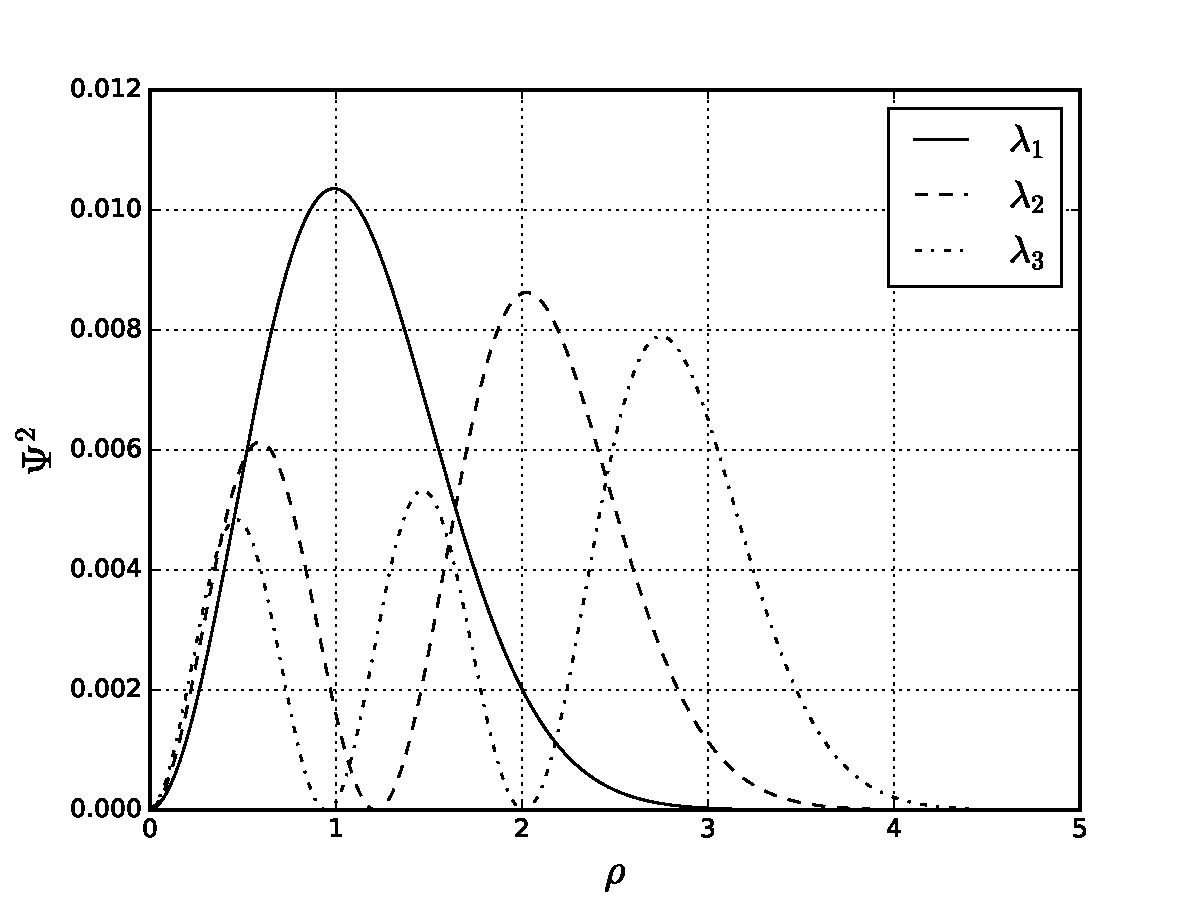
\includegraphics[scale=0.7]{one_electron}
    \caption {Probability function ($|\Psi^{2}|$) dependence from radial coordinate $\rho $ for one electron in harmonic oscillator potential.}
    \label{fig:one_electron}
  \end{center}
\end{figure}


\begin{figure}[h!] 
  \begin{subfigure}[b]{0.6\linewidth}
    \centering
    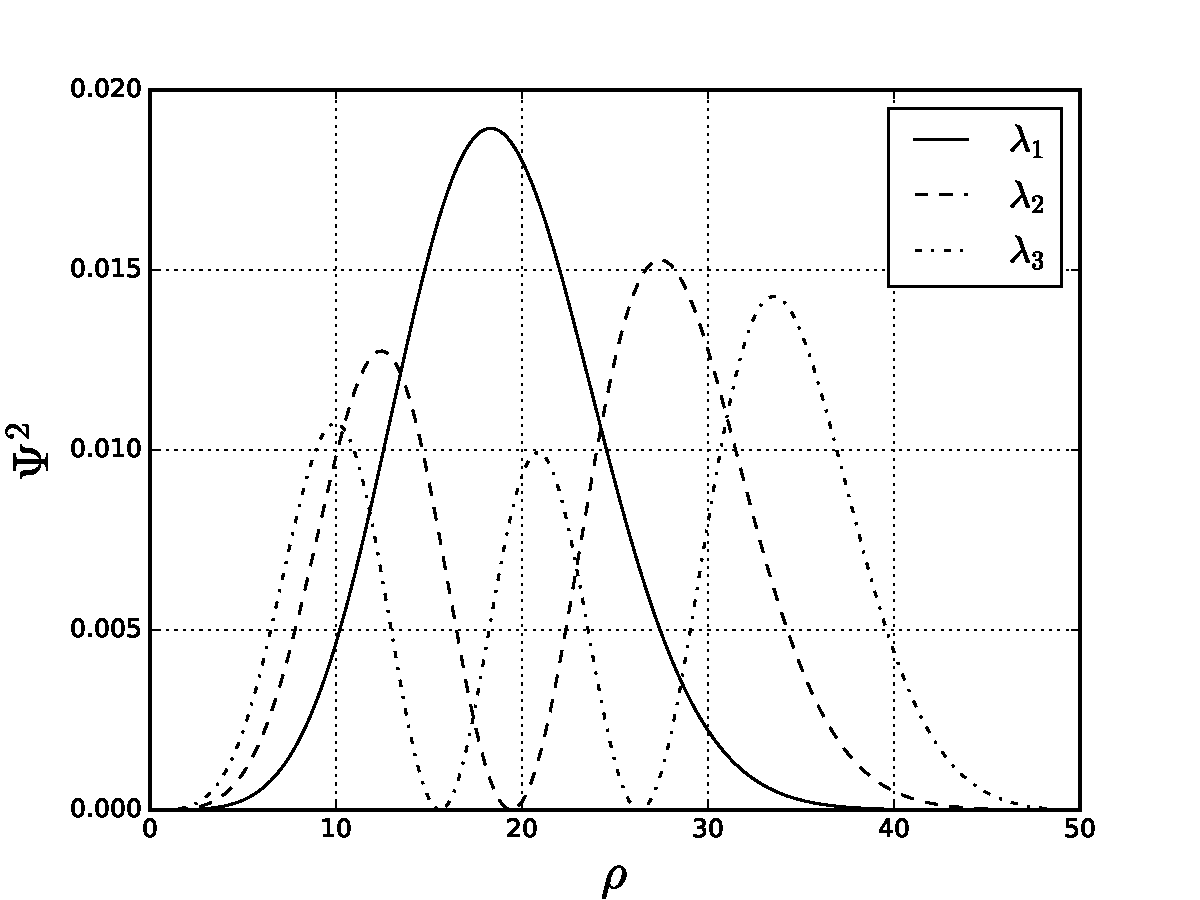
\includegraphics[width=1.1\linewidth]{two_001} 
    \caption{The $\omega$ is 0.01} 
    \label{fig1:a} 
    \vspace{1ex}
  \end{subfigure}%% 
  \begin{subfigure}[b]{0.6\linewidth}
    \centering
    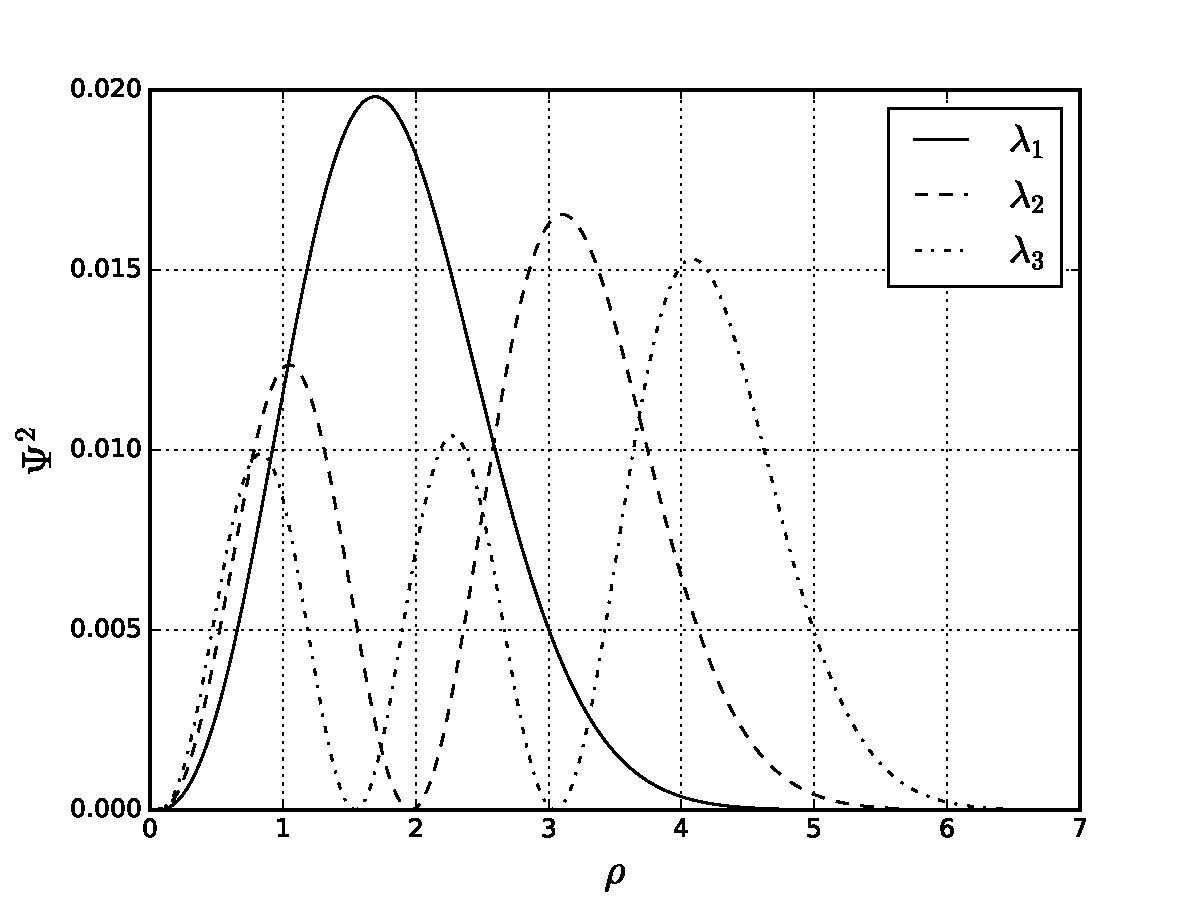
\includegraphics[width=1.1\linewidth]{two_05} 
    \caption{The $\omega$ is 0.5} 
    \label{fig1:b} 
    \vspace{1ex}
  \end{subfigure} 
  \begin{subfigure}[b]{0.6\linewidth}
    \centering
    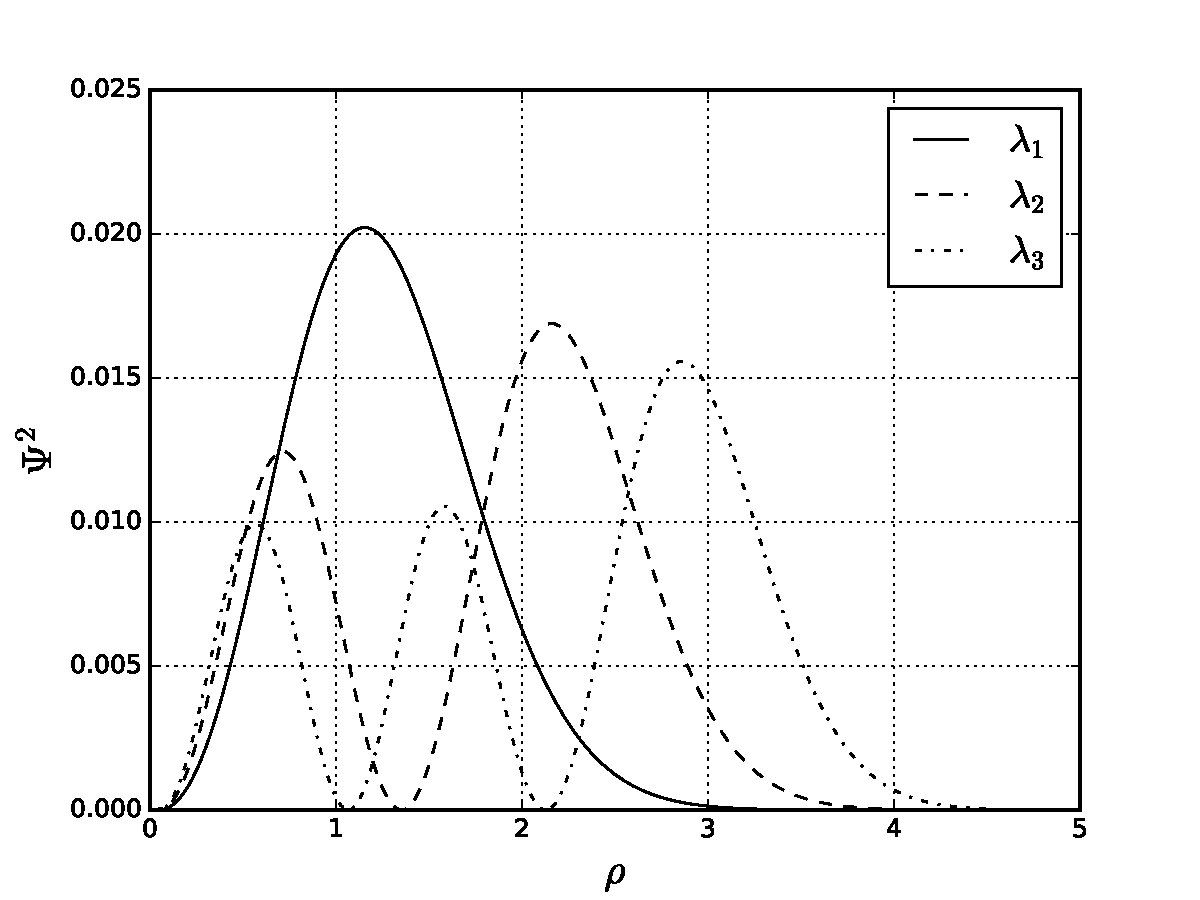
\includegraphics[width=1.1\linewidth]{two_1} 
    \caption{The $\omega$ is 1} 
    \label{fig1:c} 
  \end{subfigure}%%
  \begin{subfigure}[b]{0.6\linewidth}
    \centering
    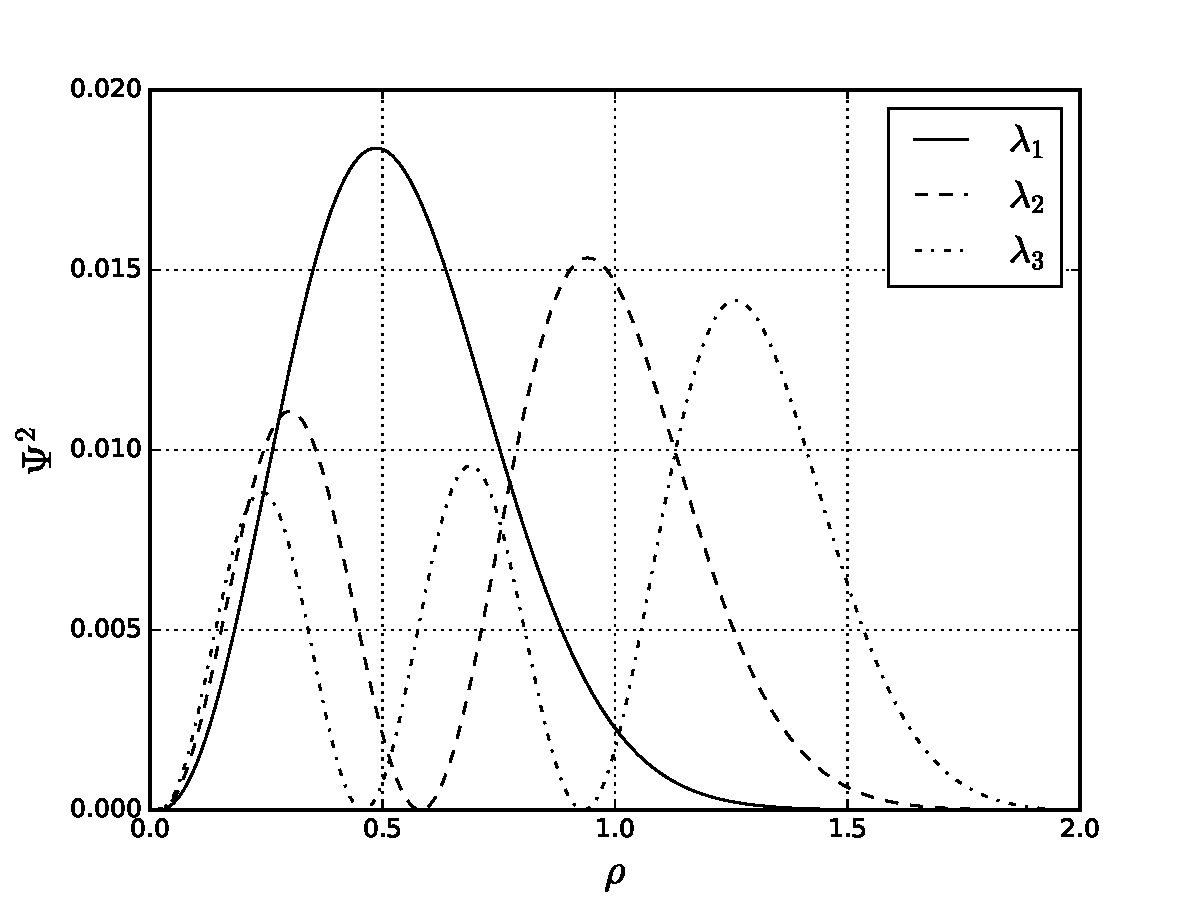
\includegraphics[width=1.1\linewidth]{two_5} 
    \caption{The $\omega$ is 5} 
    \label{fig1:d} 
  \end{subfigure} 
  \caption{ Probability functions corresponding to the three first eigenvalues for two electrons in harmonic oscillator potential without Coulomb interaction for different strengths of harmonic oscillator potential $\omega$}
  \label{fig1} 
\end{figure}



\newpage

\begin{figure}[h!] 
  \begin{subfigure}[b]{0.6\linewidth}
    \centering
    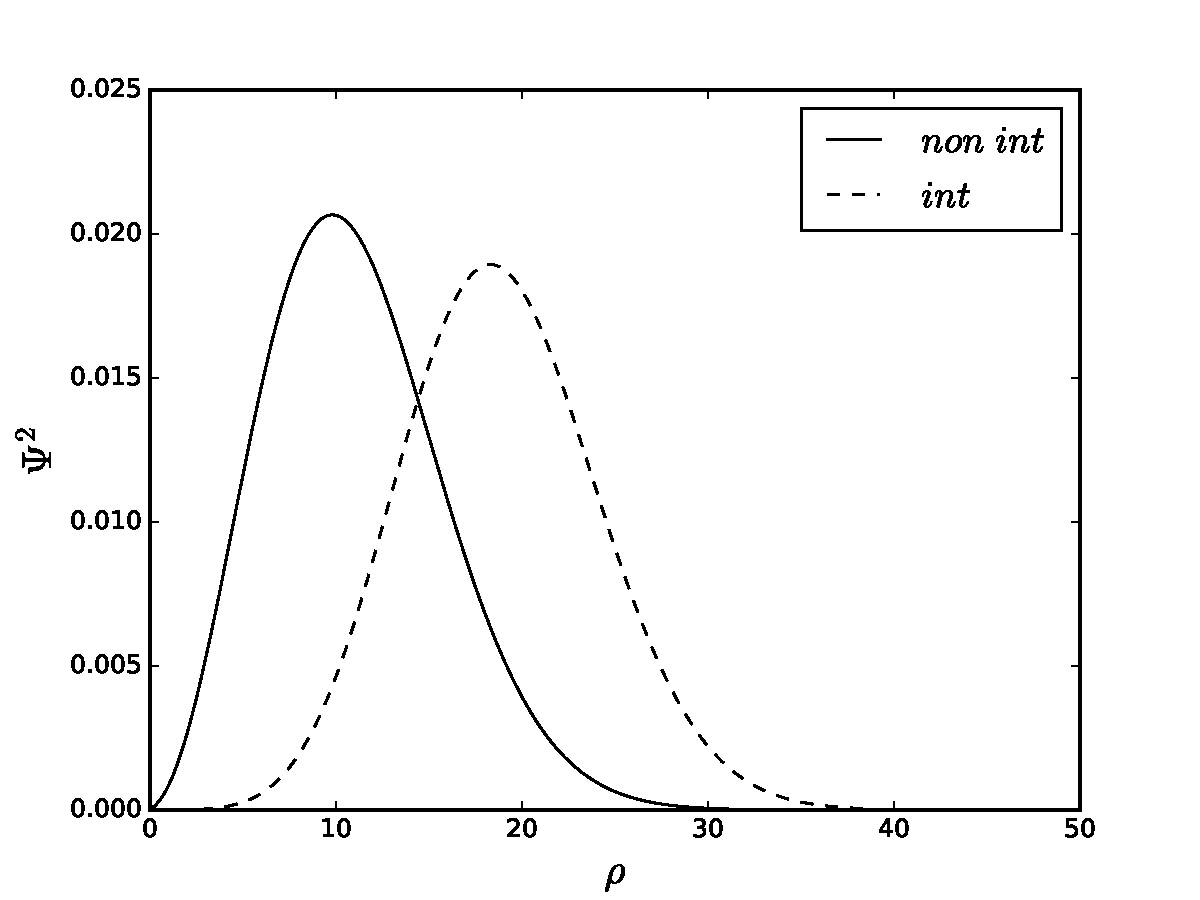
\includegraphics[width=1.1\linewidth]{two_nint_001} 
    \caption{The $\omega$ is 0.01} 
    \label{fig2:a} 
    \vspace{1ex}
  \end{subfigure}%% 
  \begin{subfigure}[b]{0.6\linewidth}
    \centering
    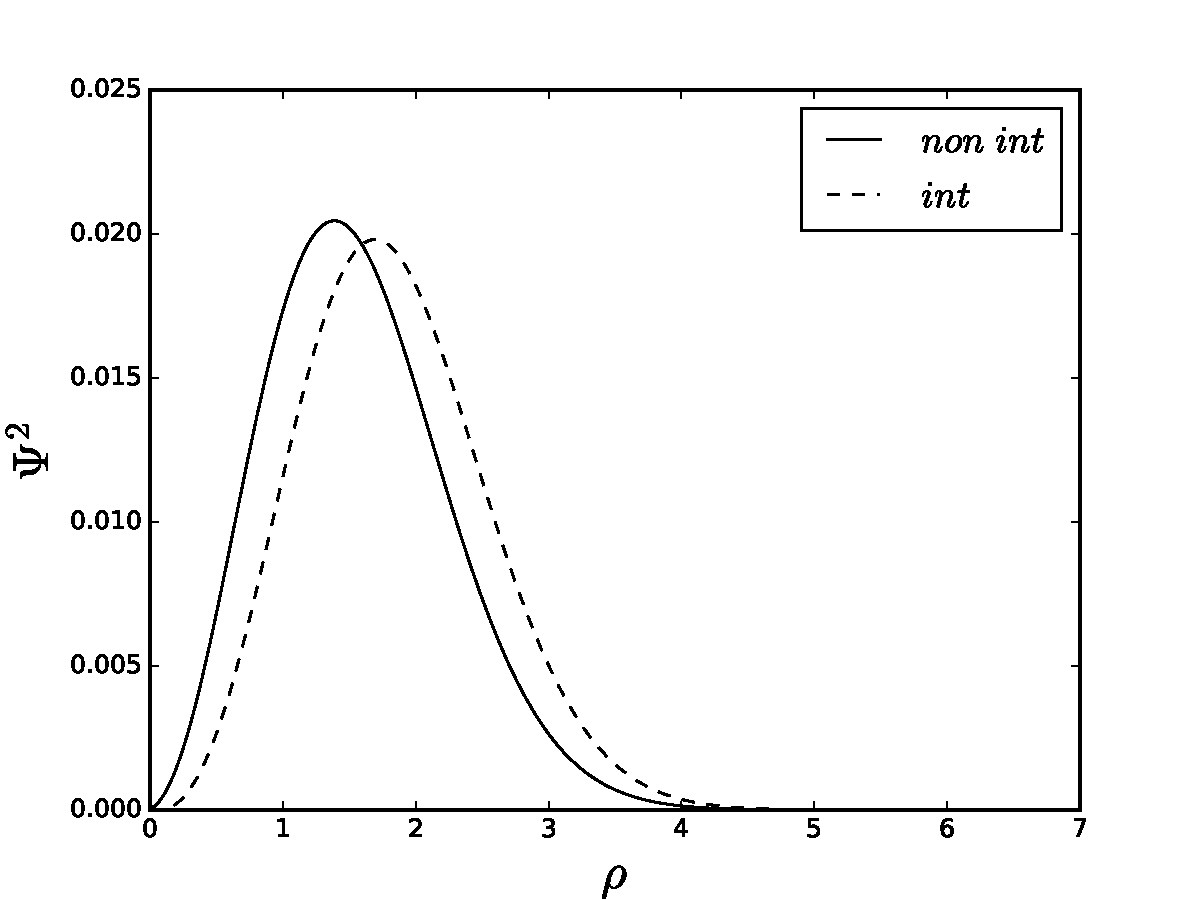
\includegraphics[width=1.1\linewidth]{two_nint_05} 
    \caption{ The $\omega$ is 0.5} 
    \label{fig2:b} 
    \vspace{1ex}
  \end{subfigure} 
  \begin{subfigure}[b]{0.6\linewidth}
    \centering
    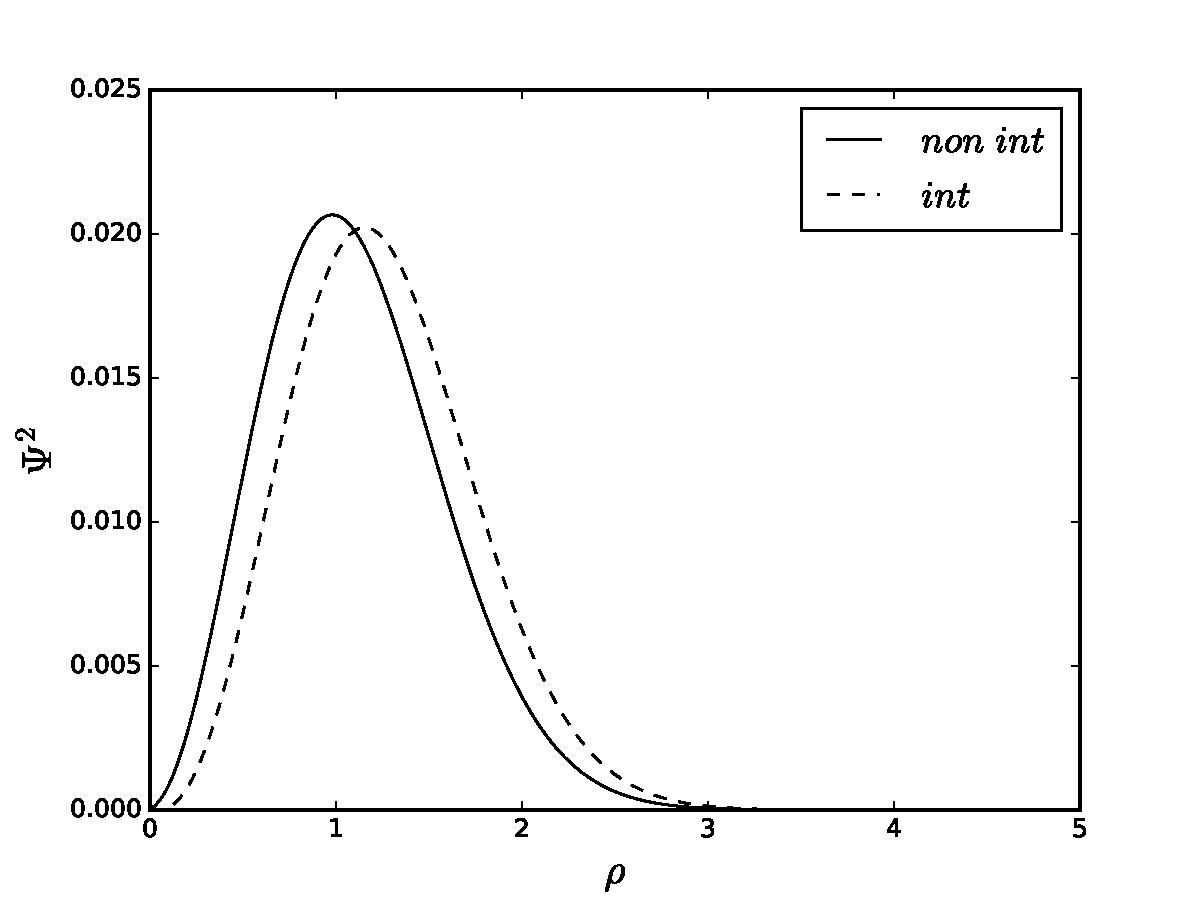
\includegraphics[width=1.1\linewidth]{two_nint_1} 
    \caption{The $\omega$ is 1} 
    \label{fig2:c} 
  \end{subfigure}%%
  \begin{subfigure}[b]{0.6\linewidth}
    \centering
    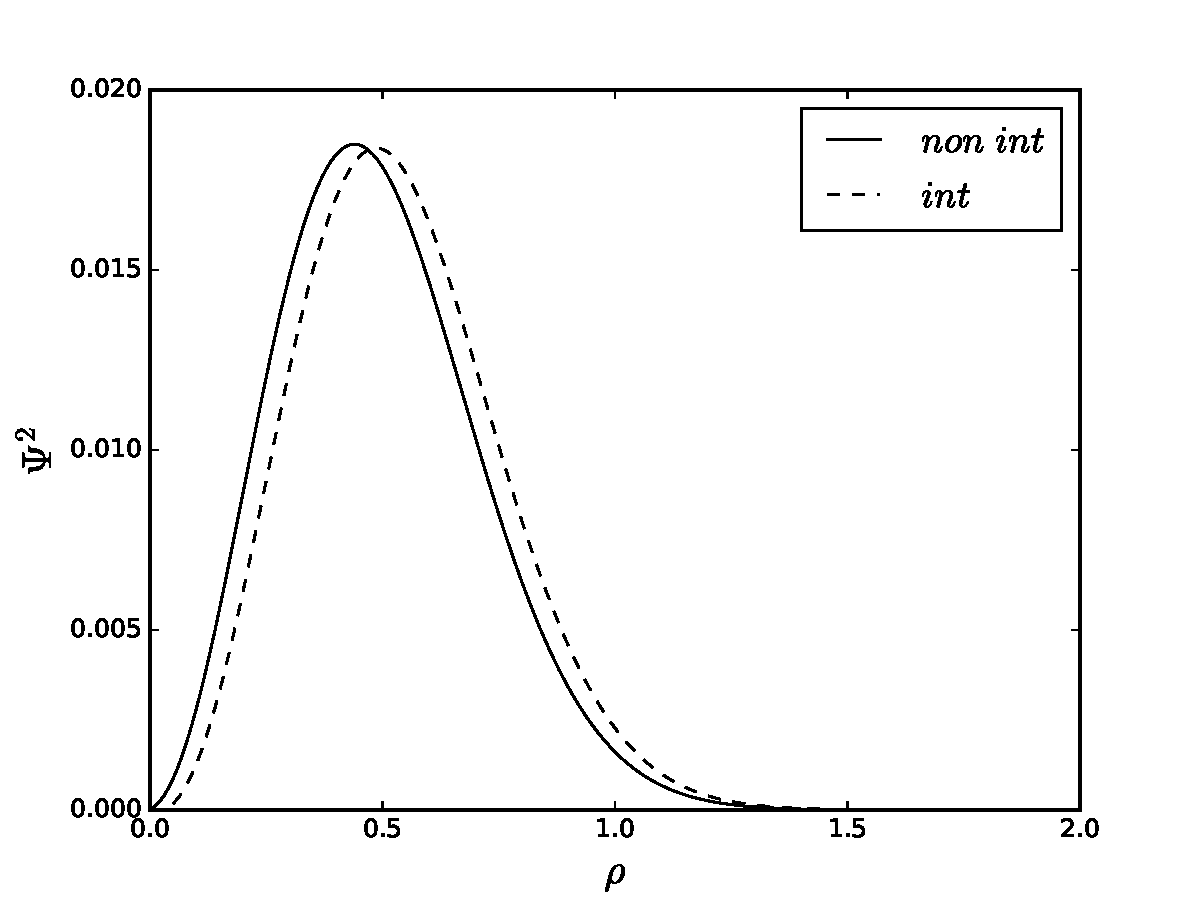
\includegraphics[width=1.1\linewidth]{two_nint_5} 
    \caption{The $\omega$ is 5} 
    \label{fig2:d} 
  \end{subfigure} 
  \caption{ Probability functions corresponding to the first eigenvalue for two electrons in harmonic oscillator potential with and without Coulomb interaction for different strengths of harmonic oscillator potential $\omega$}
  \label{fig2} 
\end{figure}


\newpage
\clearpage
\section{Conclusion and further research}\label{conc}
In this project we studied several problems. The one electron in harmonic oscillator potential, which is analytically solvable, and two electron in the harmonic oscillator potential. The latter we have studied for different strengths of harmonic oscillator. We also considered case with and without Coulomb interaction.
For the one electron case both eigenvalues and eigenvectors are in a good agreement with analytically obtained results.


\clearpage
\newpage
\begin{thebibliography}{2}
\bibitem{one} 
Morten Hjorth-Jensen. 
\textit{Computational Physics
}. 
Lecture Notes Fall 2015, August 2015.

\bibitem{two} 
W. Press, B. Flannery, S. Teukolsky, W. Vetterling 
\textit{Numerical Recipes in C++, The art of scientific Computing}. 
Cambridge University Press, 1999.

\bibitem {three}
M. Taut. 
\textit{Two electrons in an external oscillator potential: Particular analytic solutions of a Coulomb correlation problem}.
Phys. Rev. A, 11.1993.

\bibitem {four}
D. Loss, D. P. DiVincenzo
\textit{
Quantum computation with quantum dots
}
Phys. Rev. A 57, 120 – Published 1 January 1998.

\bibitem {five}
P. Patel
\textit
{The First Full-Color Display with Quantum Dots
}
MIT Technology Review, February 22, 2011. 
 
\end{thebibliography}

\end{document}
